\section{基于增量舒尔补的优化方法}

iSAM2算法\cite{kaess2008isam,kaess2012isam2}创新性地在SLAM问题中使用了贝叶斯树来编码集束优化过程中的信息矩阵分解过程,达到高效地更新平方根信息矩阵的目的,显著地提升了全局优化的性能。其算法不仅适用于SLAM中的集束优化问题,也适用于一般的非线性最小二乘问题。也正是为了保证通用性,iSAM2难以在状态之间的关联特点高度统一的SLAM问题中发挥更高的性能。

例如在图\ref{fig:sparse_matrix}中,正规方程的三维点部分(左上角部分)高度稀疏,呈对角块状,在求解时应该优先考虑这一部分的分解。iSAM2算法需要依赖COLAMD\citep{davis2004algorithm}算法来被动地检测矩阵分解的顺序,一方面需要额外的计算时间,另一方面也不一定能得到比经验更好的结果。

\subsection{舒尔补}

舒尔补(Schur complement)是一种常用的加速求解稀疏线性系统的方法,也特别适用于集束优化问题中的正规方程的求解。其本质上是基于高斯消元的分块求解线性系统的方法。对于一个集束优化问题,经过对调整变量的顺序,可以构建正规方程并求解:
\begin{equation}
    \mathrm{H} =
    \begin{bmatrix}
        \mathrm{P} & \mathrm{W}^\top \\
        \mathrm{W} & \mathrm{C}
    \end{bmatrix}, \quad
    \bm{\eta} = \begin{bmatrix} \bm{p} \\ \bm{c} \end{bmatrix}
\end{equation}
\begin{equation}
    \bm{\delta} =\mathrm{H}\setminus\bm{\eta}
\end{equation}
其中$\mathrm{P}$是三维点状态对应的信息矩阵,$\mathrm{C}$是相机状态对应的信息矩阵,$\mathrm{W}$是三维点状态和相机状态的信息矩阵。求解三维点状态和相机状态之前,先通过行变换构建舒尔补方程组:
\begin{equation}
    \left( \mathrm{C}-\mathrm{W}\mathrm{P}^{-1}\mathrm{W}^\top \right)
    \bm{\delta}_c = \bm{c}-\mathrm{W}\mathrm{P}^{-1}\bm{p}
    \label{eq:schur_complement}
\end{equation}

记舒尔补矩阵为$\mathrm{S}\doteq\mathrm{C}-\mathrm{W}\mathrm{P}^{-1}\mathrm{W}^\top$,右侧为$\bm{b}\doteq\bm{c}-\mathrm{W}\mathrm{P}^{-1}\bm{p}$。根据经验,集束优化问题中的三维点状态数量远多于相机状态数量,故矩阵$\mathrm{P}$的规模远大于舒尔补矩阵。通过求解下舒尔补方程:
\begin{equation}
    \bm{\delta}_c = \mathrm{S} \enspace\setminus\enspace \bm{b}
    \label{eq:solve_schur}
\end{equation}
可以快速得到相机状态变量的值。又因为三维点之间没有直接通过因子相连,故其信息矩阵$\mathrm{P}$呈对角块稀疏状,如图\ref{fig:sparse_matrix}所示。因此$\mathrm{P}^{-1}$矩阵的计算往往非常快速,通过变量回代又可以高效地求解剩余变量:
\begin{equation}
    \bm{\delta}_p = \mathrm{P}
    \enspace\setminus\enspace
    \left( \bm{p}-\mathrm{W}^\top\bm{\delta}_c \right)
    \label{eq:back_sub}
\end{equation}

舒尔补虽然可以大幅加速集束优化的求解,但是在标准的集束优化算法中,每一轮迭代重新构建舒尔补方程的过程仍然需要耗费大量的时间。如前面提到的,SLAM问题具有很好的局部性,每一轮求解一般都只有一小部分较新的变量有所更新,如果采用增量式的方法,每一轮迭代时只重新计算这些变量在舒尔补方程中对应的部分,则可以进一步减少计算量。

\subsection{增量舒尔补}

\begin{figure}[htb!]
    \centering
    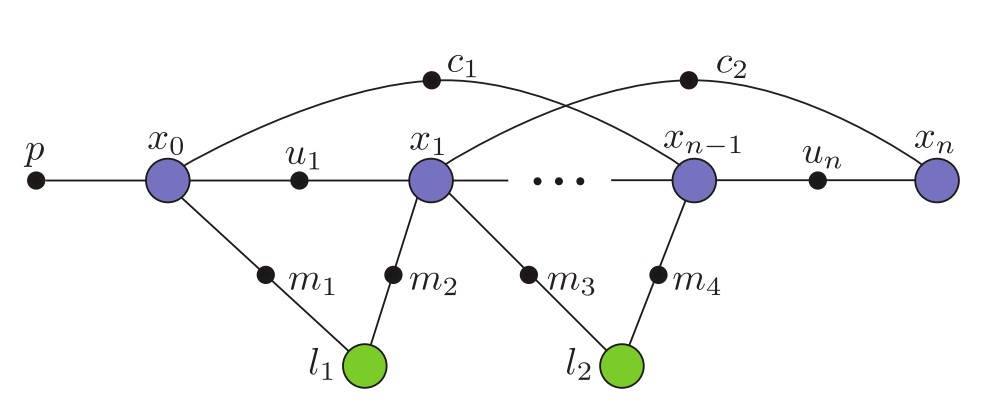
\includegraphics[width=.8\textwidth]{figs/factor_graph.png}
    \caption{因子图}
    \label{fig:factor_graph}
\end{figure}

如图\ref{fig:factor_graph}是一个常见集束优化问题的因子图示例,其对应的正规方程具有如图\ref{fig:normal_eq}所示的稀疏结构。按照式\eqref{eq:schur_complement}构建相机部分方程的舒尔补,依次迭代计算每一个三维点状态对应的舒尔补部分,并累加到图\ref{fig:reduced_sys}中的高亮部分所示的舒尔补中。图\ref{fig:schur_complement}展示了计算舒尔补的第一次迭代。

\begin{figure}[htb!]
    \centering
    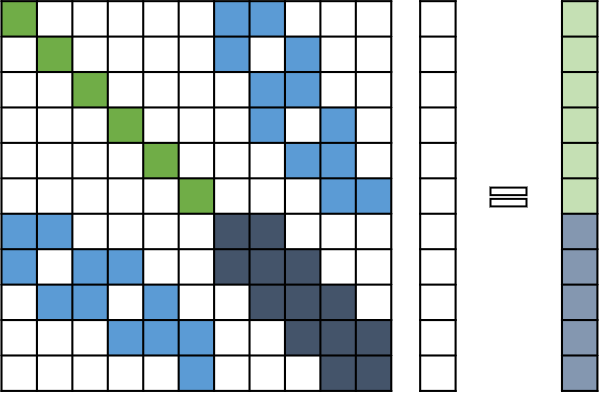
\includegraphics{figs/normal_eq.png}
    \caption{正规方程:左上角块对角矩阵部分对应三维点状态$1$至$6$的信息矩阵$\mathrm{P}$,右下角部分为相机状态$1$至$5$对应的信息矩阵$\mathrm{C}$,左下角和右上角为矩阵$\mathrm{W}$和$\mathrm{W}^\top$;中间列向量从上至下依次对应三维点状态$1$至$6$和相机状态$1$至$5$的迭代步;右侧部分从上至下依次对应三维点状态$1$至$6$和相机状态$1$至$5$。}
    \label{fig:normal_eq}
\end{figure}

\begin{figure}[htb!]
    \centering
    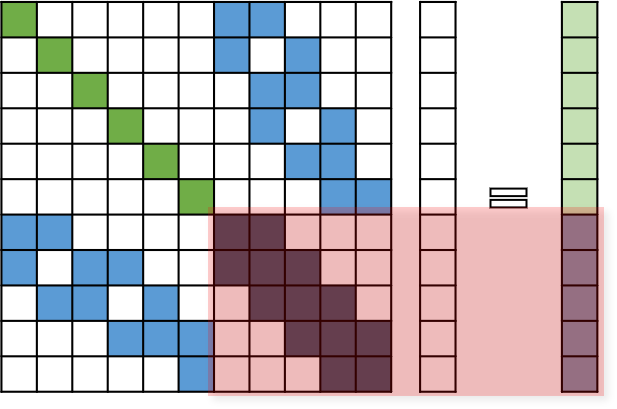
\includegraphics{figs/reduced_sys.png}
    \caption{舒尔补:高亮部分为相机状态对应舒尔补方程,其余部分为原方程。}
    \label{fig:reduced_sys}
\end{figure}

\begin{figure}[htb!]
    \centering
    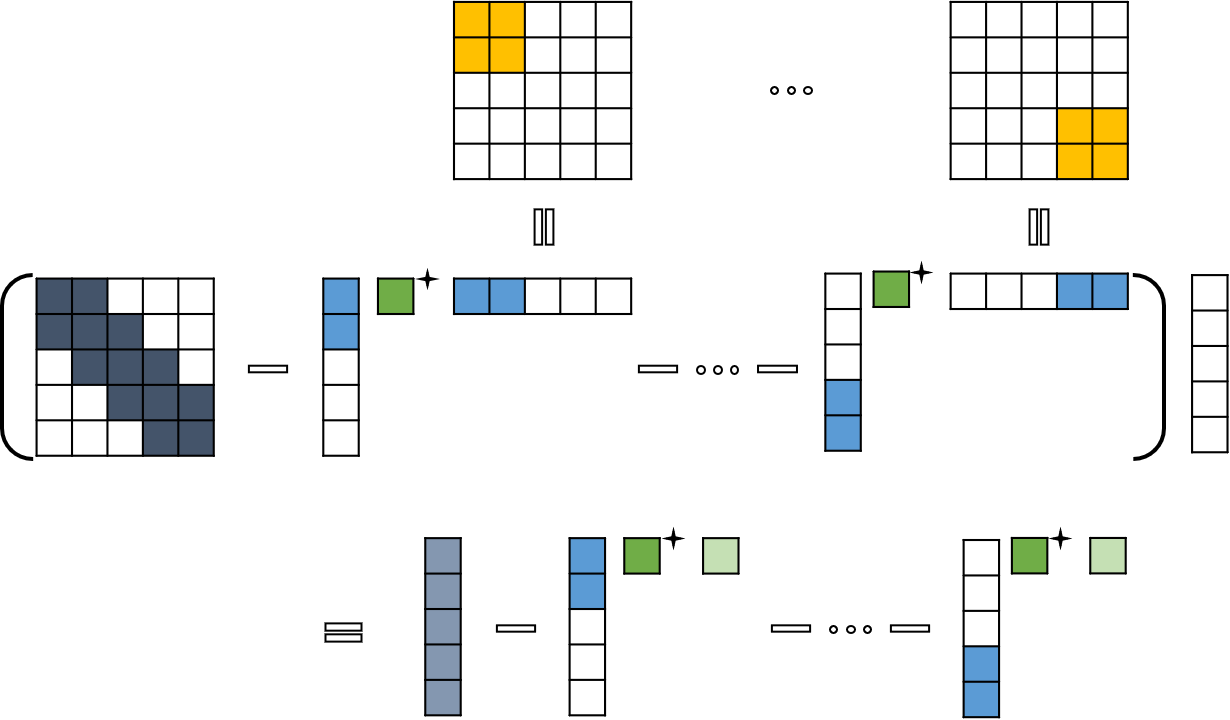
\includegraphics[width=\textwidth]{figs/schur_complement.png}
    \caption{计算舒尔补的一次迭代:从左上角开始依次迭代计算每一个三维点对应的舒尔补部分,并累加到右下角相机部分中。}
    \label{fig:schur_complement}
\end{figure}

\subsubsection{标记脏子图}

\begin{figure}[htb!]
    \centering
    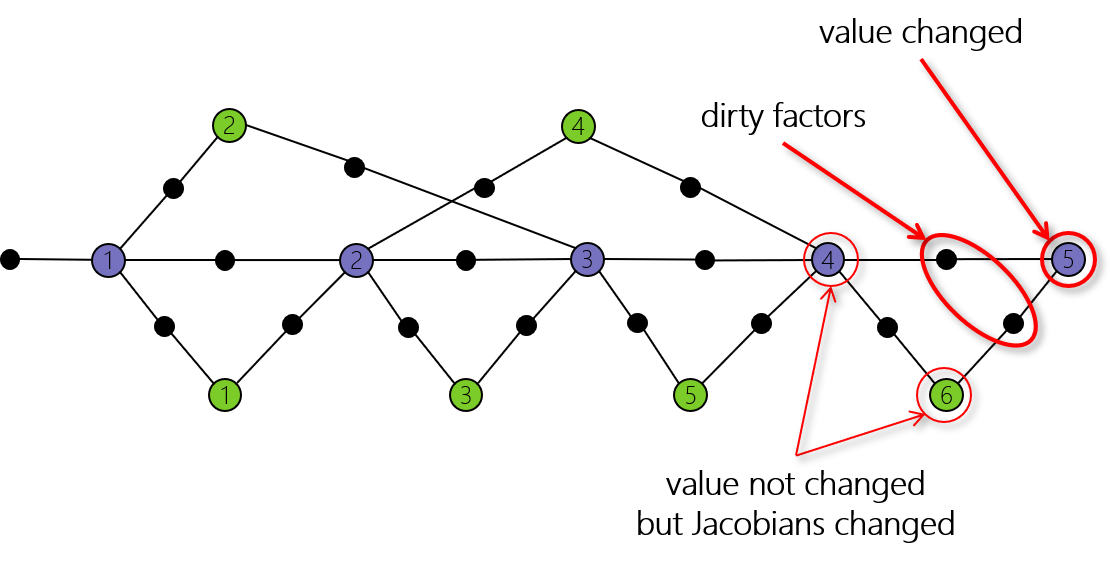
\includegraphics[width=.8\textwidth]{figs/factor_graph_dirty.png}
    \caption{因子图待更新部分:相机状态$5$为脏变量;与其直接相连的因子为脏因子;相机状态$4$和三维点状态$6$为只有梯度发生了变化的脏变量。这些节点构成了一个脏子图。}
    \label{fig:factor_graph_dirty}
\end{figure}

增量更新舒尔补的方法关键在于尽可能地复用上一次迭代的结果,只针对性地计算舒尔补方程中变化较大的变量对应的部分。以因子图\ref{fig:factor_graph}为例,假设只有相机状态$5$有较大的更新,则先将其标记为脏变量。在因子图中,只有与脏变量直接相连的因子需要标记为脏因子,如图\ref{fig:factor_graph_dirty}所示。需要注意的是,尽管相机状态$5$和三维点状态$6$的值并未发生足够大的改变,但是由于与之相邻的部分因子被标记为脏因子,因此也需要更新这些因子关于它们的雅各比矩阵。这些脏变量和脏因子共同组成了一个脏子图,对应地,图\ref{fig:normal_eq_dirty}高亮标示了舒尔补方程中需要更新的脏块。算法\ref{alg:mark_dirty}详细说明了如何通过一个简单的宽度优先搜索标记出因子图中的脏子图。

\begin{algorithm}
\caption{标记脏子图}
\begin{algorithmic}
    \Require 因子图$\check{\mathcal{G}}=\{\check{\mathcal{F}},\check{\Theta},\check{\mathcal{E}}\}$,
             迭代步长$\bm{\delta}$
    \Ensure 脏子图$\mathcal{G}=\{\mathcal{F},\Theta,\mathcal{E}\}$

    \State $\mathcal{F}\coloneqq\{\}$,
           $\Theta\coloneqq\{\}$,
           $\mathcal{E}\coloneqq\{\}$

    \ForAll{$\lVert\bm{\delta}_i\rVert \geq \varepsilon$}
        \State $\Theta\coloneqq\Theta\cup\{\bm{\theta}_i\}$
        \Comment{将变量$\bm{\theta}_i$标记为脏变量}

        \ForAll{$\bm{f}_j(\Theta_j),\bm{\theta}_i\in\Theta_j$}
            \State $\mathcal{E} \coloneqq \mathcal{E} \cup \{e_{ij}\}$
            \Comment{记录变量$\bm{\theta}_i$与因子$\bm{f}_j$相连的边$e_{ij}$}

            \State $\mathcal{F} \coloneqq \mathcal{F} \cup \{\bm{f}_j\}$
            \Comment{将因子$\bm{f}_j$标记为脏因子}
        \EndFor
    \EndFor
\end{algorithmic}
\label{alg:mark_dirty}
\end{algorithm}

\begin{figure}[htb!]
    \centering
    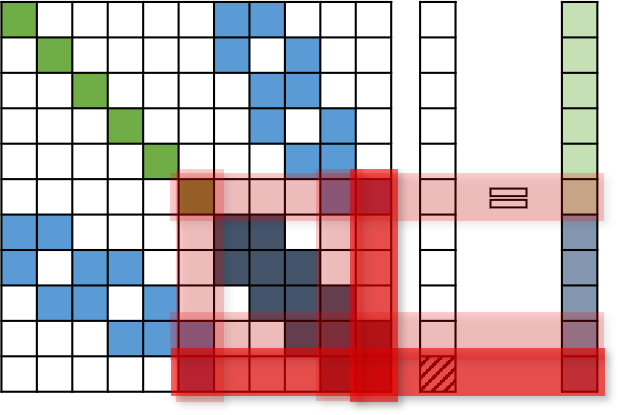
\includegraphics{figs/normal_eq_dirty.png}
    \caption{图\ref{fig:factor_graph_dirty}对应的舒尔补方程中的脏块:相机状态$4$、$5$和三维点状态$6$构成的线性子系统。}
    \label{fig:normal_eq_dirty}
\end{figure}

\subsubsection{重新计算舒尔补}

舒尔补方程中被标记为脏块的矩阵构成了一个线性子系统,对应因子图中的脏子图。如图\ref{fig:schur_update}所展示的,在增量更新舒尔补的过程中,需要先从舒尔补方程中减去脏子图的贡献,随后重新线性化所有的脏因子,最后重新计算舒尔补。算法\ref{alg:schur_update}详细描述了这个过程。需要注意的是,在计算舒尔补的过程中会重复用到$\mathrm{W}_i\mathrm{P}_{ii}^{-1}\mathrm{W}_i^\top$,$\mathrm{W}_i\mathrm{P}_{ii}^{-1}\bm{p}_i$,$\mathrm{J}_j^\top\mathrm{J}_j$,$\mathrm{J}_j^\top\bm{f}_j$,需要将这些中间项缓存下来,避免重复计算。

\begin{algorithm}
\caption{增量更新舒尔补}
\begin{algorithmic}
    \Require 脏子图$\mathcal{G}=\{\mathcal{F},\Theta,\mathcal{E}\}$,
             上一轮迭代的$\bm{\delta}$,
             $\mathrm{P}$,$\mathrm{W}$,$\mathrm{S}$,
             $\bm{p}$,$\bm{b}$
    \Ensure 更新后的
            $\mathrm{P}$,$\mathrm{W}$,$\mathrm{S}$,
            $\bm{p}$,$\bm{b}$

    \ForAll{三维点状态$\bm{\theta}_i\in{\Theta}$}
        \Comment{减去三维点对舒尔补的贡献}
        \[\begin{aligned}
                \mathrm{S} &\coloneqq \mathrm{S} + \mathrm{W}_i{\mathrm{P}_{ii}}^{-1}\mathrm{W}_i^\top \\
                \bm{b}     &\coloneqq \bm{b}     + \mathrm{W}_i{\mathrm{P}_{ii}}^{-1}\bm{p}_i
        \end{aligned}\]
    \EndFor

    \ForAll{脏因子$\bm{f}_j\in\mathcal{F}$}
        \State \Comment{减去脏因子对正规方程的贡献}
        \[\begin{aligned}
                \mathrm{H} &\coloneqq \mathrm{H} - \mathrm{J}_j^\top \mathrm{J}_j \\
                \bm{\eta}  &\coloneqq \bm{\eta} + \mathrm{J}_j^\top \bm{f}_j
        \end{aligned}\]

        \State \Comment{重新线性化脏因子}
        \[\begin{aligned}
                \mathrm{J}_j &\coloneqq \frac{\partial{\bm{f}_j(\bm{\theta}_{f_j}+\bm{\delta}_{f_j})}}
                                             {\partial{\bm{\delta}_{f_j}}} \\
                \bm{f}_j     &\coloneqq \bm{f}_j(\bm{\theta}_{f_j}+\bm{\delta}_{f_j})
        \end{aligned}\]

        \State \Comment{更新脏因子对正规方程的贡献}
        \[\begin{aligned}
                \mathrm{H} &\coloneqq \mathrm{H} + \mathrm{J}_j^\top\mathrm{J}_j \\
                \bm{\eta}  &\coloneqq \bm{\eta}  - \mathrm{J}_j^\top\bm{f}_j
        \end{aligned}\]
    \EndFor

    \ForAll{三维点状态$\bm{\theta}_i\in{\Theta}$}
        \Comment{更新三维点对舒尔补的贡献}
        \[\begin{aligned}
                \mathrm{S} &\coloneqq \mathrm{S} - \mathrm{W}_i{\mathrm{P}_{ii}}^{-1}{\mathrm{W}_i}^\top \\
                \bm{b}     &\coloneqq \bm{b}     - \mathrm{W}_i{\mathrm{P}_{ii}}^{-1}\bm{p}_i
        \end{aligned}\]
    \EndFor

\end{algorithmic}
\label{alg:schur_update}
\end{algorithm}

\begin{figure}[htb!]
    \centering
    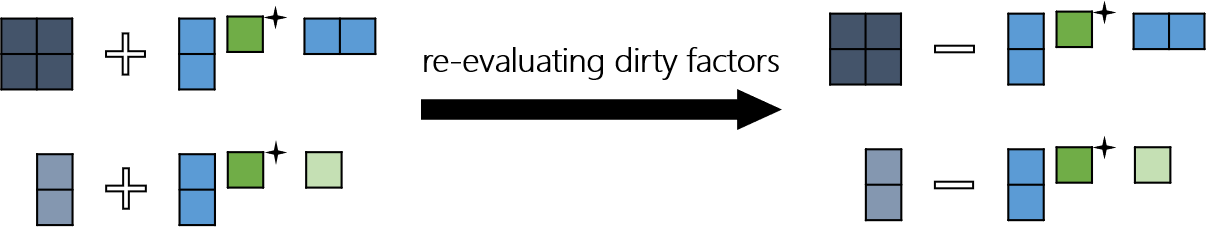
\includegraphics[width=\textwidth]{figs/schur_update.png}
    \caption{更新舒尔补}
    \label{fig:schur_update}
\end{figure}

\subsection{状态增广}

除了状态变量发生较大变化的时候需要更新因子图和舒尔补方程,集束优化过程中,如果有新的状态或因子加入,也需要对因子图进行增广,并对和舒尔补方程进行相应更新。实际上,这个过程也可以认为是算法\ref{alg:schur_update}的一个特例。如图\ref{fig:factor_graph_aug},新加入的状态通过新的因子与原因子图中相关联的部分状态共同构成了一个子图,将这个子图标记为脏子图,即可使用算法\ref{alg:schur_update}进行更新。算法\ref{alg:factor_graph_aug}给出了详细的过程,为了提高效率,因子图的增广和舒尔补方程的更新会被同时执行。

\begin{figure}[htb!]
    \centering
    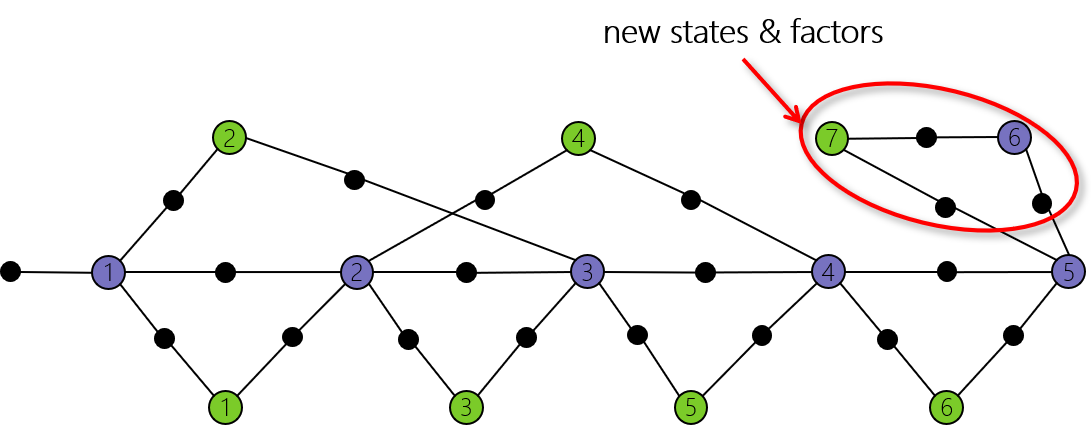
\includegraphics[width=.8\textwidth]{figs/factor_graph_aug.png}
    \caption{增广因子图}
    \label{fig:factor_graph_aug}
\end{figure}

\begin{algorithm}
\caption{状态增广}
\begin{algorithmic}
    \Require 新加入的状态和因子构成的子图
             $\check{\mathcal{G}}=\{\check{\mathcal{F}},\check{\Theta},\check{\mathcal{E}}\}$,
             上一次优化的
             $\mathrm{P}$,$\mathrm{W}$,$\mathrm{S}$,
             $\bm{p}$,$\bm{b}$
    \Ensure 增广后的因子图
            $\mathcal{G}=\{\mathcal{F},\Theta,\mathcal{E}\}$,
            和更新后的
            $\mathrm{P}$,$\mathrm{W}$,$\mathrm{S}$,
            $\bm{p}$,$\bm{b}$

    \State $\mathcal{F}\coloneqq\check{\mathcal{F}}$,
           $\Theta\coloneqq\check{\Theta}$,
           $\mathcal{E}\coloneqq\check{\mathcal{E}}$

    \ForAll{$\bm{f}_j(\Theta_j),\bm{\theta}_i\in\Theta_j$}
        \State $\mathcal{E} \coloneqq \mathcal{E} \cup \{e_{ij}\}$
        \Comment{记录变量$\bm{\theta}_i$与因子$\bm{f}_j$相连的边$e_{ij}$}

        \State $\mathcal{F} \coloneqq \mathcal{F} \cup \{\bm{f}_j\}$
        \Comment{将因子$\bm{f}_j$标记为脏因子}
    \EndFor

\end{algorithmic}
\label{alg:factor_graph_aug}
\end{algorithm}

\begin{figure}[htb!]
    \centering
    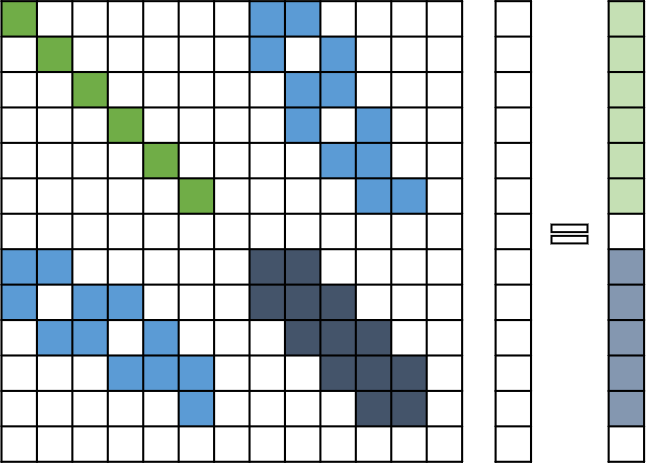
\includegraphics{figs/normal_eq_aug.png}
    \caption{增广正规方程}
\end{figure}

\begin{figure}[htb!]
    \centering
    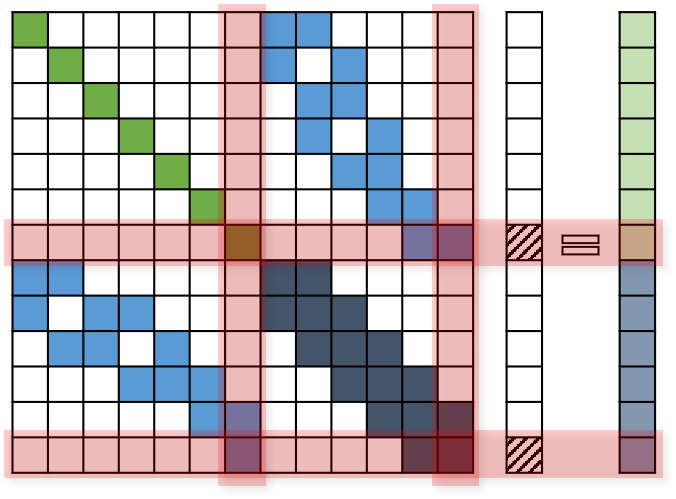
\includegraphics{figs/normal_eq_update.png}
    \caption{更新正规方程}
\end{figure}

\begin{figure}[htb!]
    \centering
    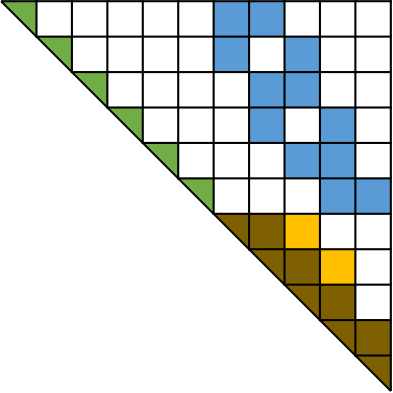
\includegraphics{figs/sqrt_info.png}
    \caption{平方根信息矩阵}
\end{figure}

\begin{figure}[htb!]
    \centering
    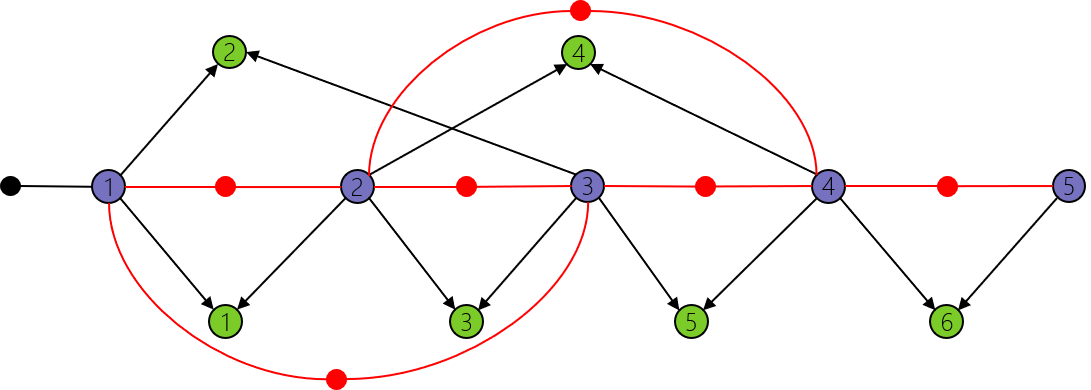
\includegraphics[width=.8\textwidth]{figs/elim.png}
    \caption{消元}
\end{figure}

\begin{figure}[htb!]
    \centering
    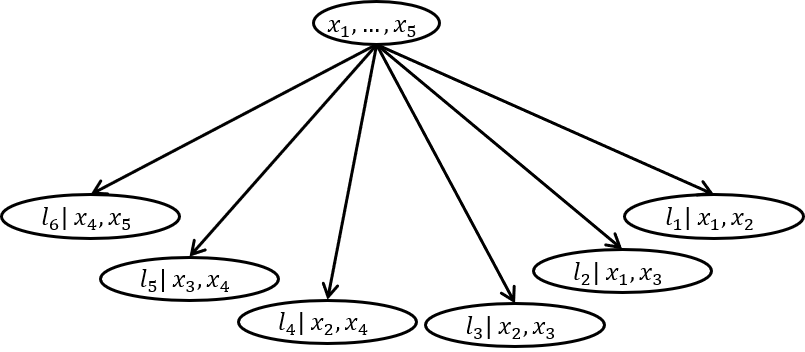
\includegraphics[width=\textwidth]{figs/bayes_tree.png}
    \caption{贝叶斯树}
\end{figure}

\begin{table}[htb!]
    \centering
    \caption{增量式集束优化算法对比:ICE-BA,SLAM++,iSAM2}
    \vspace{6pt}
    \begin{tabularx}{\textwidth}{lXXX}
               & 变量分组/排序   & 线性求解                     & 状态更新          \\ \hline
        ICE-BA & 三维点独立成组  & 增量舒尔补+共轭梯度法        & 根据步长直接判断  \\
        SLAM++ & 三维点独立成组  & 增量舒尔补+乔里斯基分解      & 根据步长直接判断  \\
        iSAM2  & CCOLAMD自动分组 & 基于贝叶树的即时线性化和求解 & 根据贝叶斯树推断  \\
    \end{tabularx}
    \label{tab:comp}
\end{table}
